\documentclass{article}

% packages for math
\usepackage{amsthm}
\usepackage{amsmath}
\usepackage{amssymb}
\usepackage{amsfonts}

% package for including images
\usepackage{graphicx}

% TAKEN FROM OVERLEAF DOCUMENTATION
% https://www.overleaf.com/learn/latex/Code_listing
\usepackage{listings}
\lstset{language=Python}
\usepackage{xcolor}
\definecolor{codegreen}{rgb}{0,0.6,0}
\definecolor{codegray}{rgb}{0.5,0.5,0.5}
\definecolor{codepurple}{rgb}{0.58,0,0.82}
\definecolor{backcolour}{rgb}{0.95,0.95,0.92}
\lstdefinestyle{mystyle}{
  backgroundcolor=\color{backcolour},
  commentstyle=\color{codegreen},
  keywordstyle=\color{magenta},
  numberstyle=\tiny\color{codegray},
  stringstyle=\color{codepurple},
  basicstyle=\ttfamily\footnotesize,
  breakatwhitespace=false,
  breaklines=true,
  captionpos=b,
  keepspaces=true,
  numbers=left,
  numbersep=5pt,
  showspaces=false,
  showstringspaces=false,
  showtabs=false,
  tabsize=2
}
\lstset{style=mystyle}

% environment for solutions
\theoremstyle{remark}
\newtheorem*{solution}{Solution}

% capital letters for problem parts
\renewcommand{\theenumi}{\Alph{enumi}}

% no page numbers
\pagenumbering{gobble}

% UNCOMMENT IF YOU DON'T WANT PROBLEMS ON INDIVIDUAL PAGES
% \renewcommand{\pagebreak}{}

\newcommand{\vv}[1]{\mathbf{#1}}
\newcommand{\R}{\mathbb R}
\DeclareMathOperator{\vspan}{span}
\DeclareMathOperator{\cod}{cod}
\DeclareMathOperator{\ran}{ran}
\DeclareMathOperator{\col}{Col}
\DeclareMathOperator{\nul}{Nul}
\DeclareMathOperator{\rank}{rank}

\title{
  Homework 10
}
\author{CAS CS 132: Geometric Algorithms}
\date{Due: \textbf{Thursday November 23, 2023 at 11:59PM}}

\begin{document}
\maketitle

\subsection*{Submission Instructions}
\begin{itemize}
\item Make the answer in your solution to each problem abundantly clear (e.g., put a box around your answer or used a colored font if there is a lot of text which is not part of the answer).
\item Choose the correct pages corresponding to each problem in Gradescope. Note that Gradescope registers your submission as soon as you submit it, so you don't need to rush to choose corresponding pages.
  \textbf{For multipart questions, please make sure each part is accounted for.}
\end{itemize}
Graders have license to dock points if either of the above instructions are not properly followed.


\section*{Practice Problems}

The following list of problems comes from \textit{Linear Algebra and its Application 5th Ed} by David C.\ Lay, Steven R.\ Lay, and Judi J.\ McDonald.
They may be useful for solidifying your understanding of the material and for studying in general.
\textbf{They are optional, so please don't submit anything for them}.

\begin{itemize}
\item 5.3.1, 5.3.3, 5.3.6, 5.3.9, 5.3.11, 5.3.26, 5.3.27, 5.3.28
\end{itemize}

\pagebreak
\section{Diagonalization by Computation}

(20 points) Find a diagonalization $PDP^{-1}$ of the following matrix
\begin{displaymath}
  \begin{bmatrix}
    0 & 2 & 2 \\
    5 & -6 & -5 \\
    -9 & 12 & 11
  \end{bmatrix}
\end{displaymath}
You should use Python to do this, and you should include the lines of code you used.
Furthermore, the diagonal entries of $D$ should be in decreasing order from left to right and the \textbf{entries of $P$ should be integers}.
In particular, you can't directly use the eigenvectors given to you by \texttt{numpy.linalg.eig} (though you can use the eigenvalues).

\medskip

\begin{solution}
\end{solution}

\pagebreak
\section{$2\times 2$ Matrices and Diagonalization}

Consider an arbitrary $2 \times 2$ matrix
\begin{displaymath}
  A =
  \begin{bmatrix}
    a & b \\
    c & d
  \end{bmatrix}
\end{displaymath}

\begin{enumerate}
\item (8 points)
  Find an expression for the characteristic polynomial of $A$.
  In other words, supposing that $i\lambda^2 + j\lambda + k$ is the characteristic polynomial of $A$, find expressions for $i$, $j$, and $k$ in terms of $a$, $b$, $c$, and $d$.
\item (8 points)
  Recall that for a quadratic polynomial $p(x) = ix^2 + jx + k$, the discriminant $j^2 - 4ik$ tells us how many roots $p$ has: $p$ has $0$, $1$ or $2$ roots if the discriminant is less than $0$, equal to $0$, or greater than $0$, respectively.
  Use this to derive an expression $E$ in terms of $a$, $b$, $c$, and $d$ where $A$ has $0$, $1$, or $2$ eigenvalues if $E < 0$, $E = 0$, or $E > 0$, respectively.
\item (4 points) Using your expression in part B, argue that \textit{every $2 \times 2$ matrix with positive entries has two distinct eigenvalues.}
  Note that this implies every $2 \times 2$ matrix with positive entries is diagonalizable.
  \textit{Hint.} Try to write your expression in Part B so that it is of the form `$(\square - \square)^2 + 4\square\square$' and reason about why this must be positive.
\end{enumerate}
\medskip

\begin{solution}
\end{solution}

\pagebreak
\section{PageRank (Programming)}

(40 points) There is no fun (at least in my opinion) in learning about PageRank and never trying it out on really big graphs, where naive implementations don't work.
In this problem, you'll be filling in some of the core functionality of an implementation of PageRank that can be applied to graphs with millions of edges.

I understand that these instructions are long, but \textbf{please read through them carefully and entirely.}
They are formatted so that you \textit{could} build this program from the ground up if you wanted to, but a lot of it is implemented for you.
There are \textbf{Tasks} associated with step which detail the actual code you need to write.

\subsection*{Part 0: Setting Up}

When doing ``real world'' computational linear algebra it is often better to depend on libraries written by experts.
We will be using two Python packages in addition to SciPy and NumPy:
\begin{itemize}
\item
  \textbf{NetworkX}\footnote{\texttt{https://networkx.org}} is a package for working with and analyzing graphs.
  It is very fast and has a nice interface for turning graphs into matrices.
\item
  \textbf{scikit-learn}\footnote{\texttt{https://scikit-learn.org/stable/}} is a package for machine learning.
  Perhaps unsurprisingly, it has a lot of very useful functions for working with matrices.
  It is certainly worth exploring, but we will only need one function from it.
\end{itemize}

\smallskip
\noindent
\textbf{Task.}
You will have to install these packages in order to use them.
I would recommend using pip via the following commands:
\begin{lstlisting}
python3 -m pip install networkx
python3 -m pip install scikit-learn
\end{lstlisting}
You may have to replace \texttt{python3} with \texttt{python} or \texttt{py} depending your system.
You should then be able to verify that they are install by opening a Python interpreter and typing
\begin{lstlisting}
import networkx
import sklearn
\end{lstlisting}
\textbf{Please try this early.} The course staff is willing to help you in office hours, but it will be hard to manage the closer we get to the deadline.
Also note there are many Stack Overflow and blog posts about install packages with \texttt{pip} for IDEs like Spyder,\footnote{ \texttt{https://stackoverflow.com/questions/63109860/how-to-install-python-packages-for-spyder}} so don't hesitate to do some Googling.

\subsection*{Part 1: Loading Graphs}
We will be loading textual representations of graphs in \textit{adjacency list format} (\texttt{.adjlist}) into our program.
The format is simple, each line represents an edge and contains two numbers, each representing the nodes connected by the edge.
A line of the form
\begin{lstlisting}
i j
\end{lstlisting}
represents an edge from node \texttt{i} to \texttt{j}.
So a file containing
\begin{lstlisting}
0 1
1 2
2 0
\end{lstlisting}
represents a directed triangle graph (note that nodes are 0-indexed).
See the NetworkX documentation for more details.\footnote{\texttt{https://networkx.org/documentation/stable/reference/readwrite/adjlist.html}}
There is a NetworkX function called \texttt{read\_adjlist} which we will use to read graphs into our program.

\smallskip
\noindent
\textbf{Task.}
You should take a look at the file \texttt{basic.adjlist}, which represents the graph that we saw in lecture:
\begin{center}
  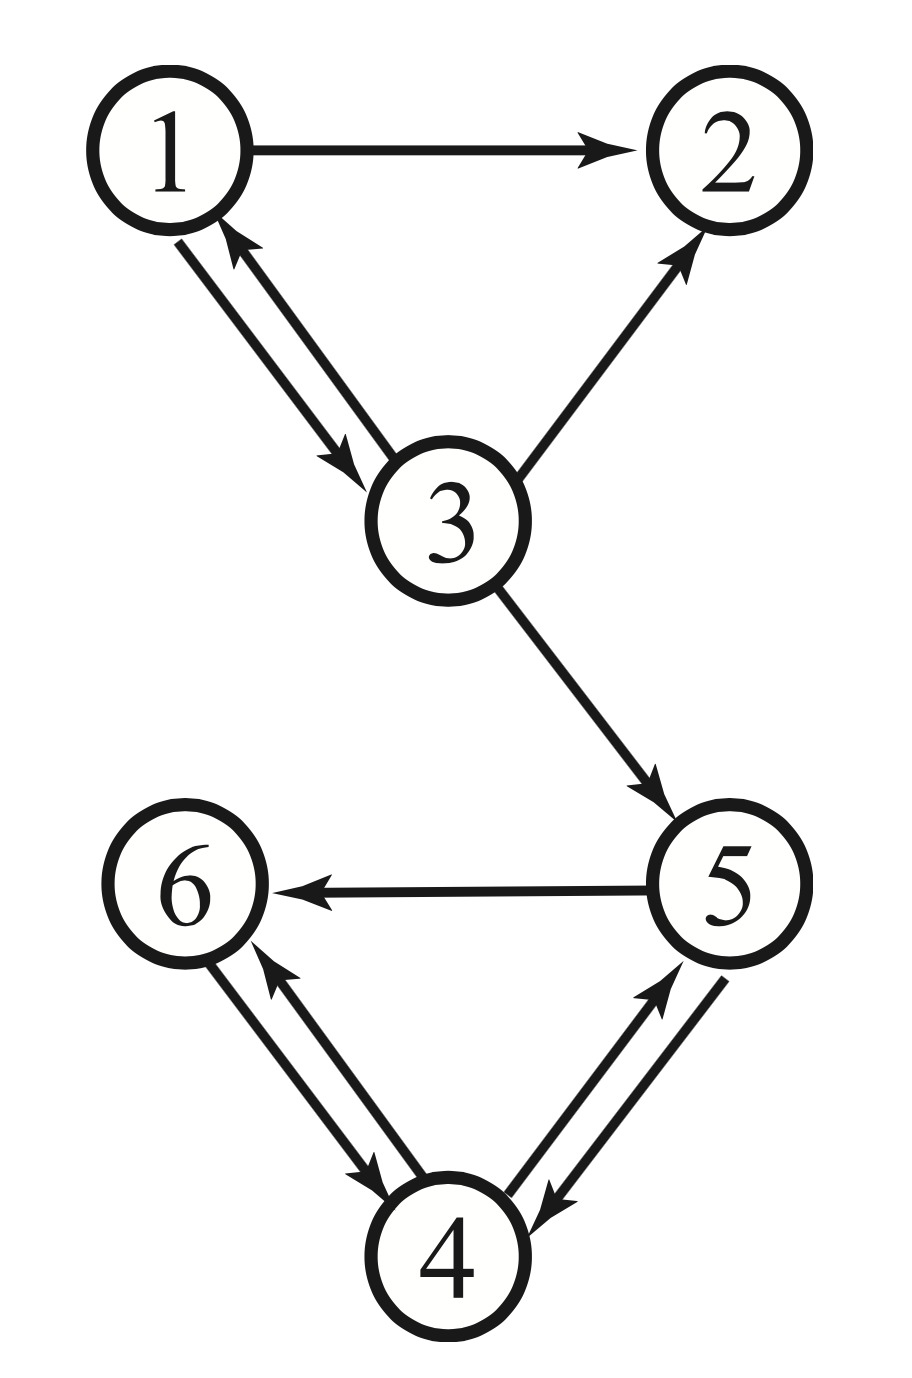
\includegraphics[width=1in]{deeper-pagerank-fig.jpg}
\end{center}
Note that \textbf{nodes are 0-indexed} in this representation so this file has values from 0 to 5.
You will be using this file for testing.

\subsection*{Part 2: Building Sparse Adjacency Matrices}

So far in this course, we've been working with NumPy arrays to represent matrices, but NumPy arrays require too much space to represent very large matrices.
We saw on a previous assignment that matrices from practical applications can sometimes be \textit{sparse}, in that they don't have very many entries relative to their size.
This is the case for many adjacency matrices.

In SciPy, there are a number of implementations of sparse matrices which are more space efficient and more efficient to manipulate than standard NumPy arrays.
In NetworkX there is a function called \texttt{adjacency\_matrix} which builds an adjacency matrix in one of these sparse implementations.

\smallskip
\noindent
\textbf{Task.}
Run the command \texttt{python3 pagerank.py basic.adjlist 2}.
This will throw an error since you have not implemented the power method yet, but you should see printed the adjacency list for the above graph. Make sure that it looks correct.

\subsection*{Part 3: Normalizing Sparse Matrices}

In Homework 6, we had an opportunity to write a function which converted an adjacency matrix into a transition matrix.
That implementation is (surprise surprise) too slow to work with very large sparse matrices.
This is quite a difficult problem, which is why there is a scikit-learn function called \texttt{normalize} for doing this.
We will use this out of the box.

\smallskip
\noindent
\textbf{Task.} After running the same command as in the previous step, you should also see the normalized form of the adjacency matrix. Make sure that it looks correct.

\subsection*{Part 4: One Step of the Power Method}

The bulk of your work is going to be in defining the function which does one iteration of the power method.
The reason this part is tricky is that we cannot do boundary reflecting or damping \textit{within the matrix} as we did in lecture.
This is because both boundary reflecting and damping \textbf{make the matrix dense} which would defeat the purpose of this using the sparse matrix in the first place.

The key observation is that both boundary reflecting and damping can be implemented without changing the very large sparse normalized matrix.
The equation that we used in lecture for the final transition matrix was
\begin{displaymath}
  (1 - \alpha)A + \frac{\alpha}{n}\mathsf 1
\end{displaymath}
where $A$ is the normalized matrix with all-zeros columns replaced with all-ones columns (before normalization).\footnote{Historically $(1 - \alpha)$ is called the \textit{damping factor} and the original paper on PageRank takes $\alpha$ to be $0.15$ (we will do the same).}
The first step is to notice that $A$ can be thought of as the matrix $A' + \frac{1}{n}A_z$ where $A'$ is the normalized matrix possibly with all-zeros columns and $A_z$ is the matrix with all-ones columns where $A'$ has all-zeros columns and zeros everywhere else. In the context of our running example:
\begin{displaymath}
  \begin{bmatrix}
    0 & 1/6 & 1/3 & 0 & 0 & 0 \\
    1/2 & 1/6 & 1/3 & 0 & 0 & 0 \\
    1/2 & 1/6 & 0 & 0 & 0 & 0 \\
    0 & 1/6 & 0 & 0 & 1/2 & 1 \\
    0 & 1/6 & 1/3 & 1/2 & 0 & 0 \\
    0 & 1/6 & 0 & 1/2 & 1/2 & 0
  \end{bmatrix}
\end{displaymath}
is the same as
\begin{displaymath}
  \begin{bmatrix}
    0 & 0 & 1/3 & 0 & 0 & 0 \\
    1/2 & 0 & 1/3 & 0 & 0 & 0 \\
    1/2 & 0 & 0 & 0 & 0 & 0 \\
    0 & 0 & 0 & 0 & 1/2 & 1 \\
    0 & 0 & 1/3 & 1/2 & 0 & 0 \\
    0 & 0 & 0 & 1/2 & 1/2 & 0
  \end{bmatrix}
  +
  \frac{1}{6}
  \begin{bmatrix}
    0 & 1 & 0 & 0 & 0 & 0 \\
    0 & 1 & 0 & 0 & 0 & 0 \\
    0 & 1 & 0 & 0 & 0 & 0 \\
    0 & 1 & 0 & 0 & 0 & 0 \\
    0 & 1 & 0 & 0 & 0 & 0 \\
    0 & 1 & 0 & 0 & 0 & 0 \\
  \end{bmatrix}
\end{displaymath}
Next, we're not actually interested in the above matrix, but the matrix-vector multiplication
\begin{displaymath}
  ((1 - \alpha)A + \frac{\alpha}{n}\vv 1)\vv v
\end{displaymath}
for some vector $\vv v$, which can be rewritten as
\begin{displaymath}
  (1 - \alpha)A'\vv v + \frac{1 - \alpha}{n}A_z\vv v +  \frac{\alpha}{n}\vv 1 \vv v
\end{displaymath}
and the two vectors on the right in this equation have a very simple structure.

\smallskip
\noindent
\textbf{Task.}
You will be implementing a single step of the power method in the function \texttt{power\_step}.
Given a sparse matrix \texttt{A'} and a 2D NumPy array \texttt{v}, you need to implement the
equation
\begin{displaymath}
  (1 - \alpha)A'\vv v + \frac{1 - \alpha}{n} A_z\vv v +  \frac{\alpha}{n}\vv 1 \vv v
\end{displaymath}
\textit{without} building the matrices $A_z$ or $\frac {\alpha}{n}\vv 1$.
You cannot, for example, use\footnote{This is not a restriction of the assignment, this matrix will be too large to build on your machine.}
\begin{displaymath}
  \texttt{(alpha / A'.shape[0]) * np.ones(A'.shape)}
\end{displaymath}
Instead, you need to think about what the vectors $\frac{1 - \alpha}{n}A_z\vv v$ and $\frac{\alpha}{n}\vv 1 \vv v$ are, and compute that separately.
For the first of these two, you are given a vector \texttt{zero\_cols} as input which has the property that $\texttt{zero\_cols[i]}$ is $1$ if the $i$th column of $A'$ is all-zeros, and $0$ otherwise.

\textbf{This is probably the trickiest part, so give it some thought}. A couple last implementation notes:
\begin{itemize}
\item
  You should \textbf{not} use the \texttt{A @ v} for matrix-vector multiplication when \texttt{A} is sparse, but rather \texttt{A.dot(v)}.
  This is better optimized for sparse matrices.
\item
  Remember that adding a number to a vector adds that number entry-wise.
  For example, \texttt{np.array([1, 2, 3]) + 2 * np.ones(3)} is the same as \texttt{np.array([1, 2, 3]) + 2} is the same as \texttt{np.array([3, 4, 5])}.
\end{itemize}

\subsection*{Part 5: Power Method}

Now that we have pre-processed our matrix and built the function for doing an iteration of our power method, we can implement the power method itself.
This is a matter of implementing the psuedocode from lecture and the notes.

\smallskip
\noindent
\textbf{Task.}
You will be implementing the power method in the function \texttt{power\_iter}.
You should separately write the function \texttt{l1\_error} which computes the function
\begin{displaymath}
  \mathsf{error}_{\ell^1}(\vv u, \vv v) = \sum_{i = 1}^n |\vv u_i - \vv v_i|
\end{displaymath}
as in the notes.
If you're interested in where the name comes from, feel free to peruse the Wikipedia page on Norms.\footnote{\texttt{https://en.wikipedia.org/wiki/Norm\_(mathematics)\#Euclidean\_norm}}

You'll notice when you run the \texttt{pagerank.py} program a bunch of stuff is printed to the command line.
In this function you \textbf{must} call the \texttt{print\_error\_log} once every 10 iterations of the power method, and one last time when you stop iterating (so you can see the final error).
For example, a run might print the following.
\begin{lstlisting}
    | error after 10 iterations: 0.03154451079478763
    | error after 20 iterations: 0.003705951856289287
    | error after 30 iterations: 0.0005351506008266042
    | error after 40 iterations: 8.340084685614549e-05
    | error after 50 iterations: 1.3684642707116416e-05
    | error after 60 iterations: 2.3141829071034e-06
    | error after 70 iterations: 3.9985909018511144e-07
    | error after 80 iterations: 7.079267907127914e-08
    | error after 90 iterations: 1.2740109503149871e-08
    | error after 92 iterations: 9.043053349643915e-09
\end{lstlisting}
So all together, the run took 92 iterations.
This will make it easier for you to see the progress that is being made as you run it.

\subsection*{Part 6: Running PageRank}

When you're done, you will be able to run your program on large graphs taken from the Stanford Large Network Dataset Collection.\footnote{\texttt{http://snap.stanford.edu/data/index.html}}
The assignment comes with three graphs based on actual Web data, one from Stanford, one from Stanford and Berkeley, and one from Google.

You will be filling in functions in the file \texttt{hw10prog.py}, but the actual program for PageRank is \texttt{pagerank.py}.
This file imports the functions that you write.
\textbf{You should read through \texttt{pagerank.py} and try to understand what's going on to the best of your ability.}
It's okay if you don't get everything.

The file \texttt{pagerank.py} takes two arguments at the command line: the name of a file in adjacency list format, and an exponent for the error tolerance used in the power method.
So
\begin{lstlisting}
  python pagerank.py basic.adjlist 4
\end{lstlisting}
will run PageRank on the graph in \texttt{basic.adjlist} with error tolerance $0.0001$.
If you type
\begin{lstlisting}
  python pagerank.py
\end{lstlisting}
with no arguments, you will get a usage string that gives you more detail on this.

You can do this problem by running the program in this way, but the project also comes with a Makefile.
If you haven't had a chance to work with Makefiles, they are used to organize code building, running and cleaning processes.
On the command line, you can instead just run the following commands:
\begin{itemize}
\item \texttt{make basic} runs PageRank on the basic graph from the running example
\item \texttt{make stanford} runs PageRank on the Stanford web data
\item \texttt{make berkstan} runs PageRank on the Berkeley-Stanford data
\item \texttt{make google} runs PageRank on the Google data
\item \texttt{make fullrun} runs PageRank on all three of the large graphs
\item \texttt{make destroy} deletes all auxiliary files created by the program (more on this in a moment)
\end{itemize}
The last thing you need to know about running the program: you'll find that preprocessing will take the bulk of the time when running.
To make this a bit easier, the program saves intermediate representations of the pre-processed graphs and rankings it finds so that you don't have to recompute them if you rerun the program.
These are the files with the extensions \texttt{.npy} and \texttt{.npz}.
So \textbf{if you find that your implementation is incorrect but you already ran it} you have to delete these files or call \texttt{make destroy} to get rid of them before recomputing the ranking.

\smallskip
\noindent
\textbf{Task.}
You should run PageRank on every large graph with an error tolerance of $10^{-8}$.
Alternatively, you can use \texttt{make fullrun}.
You should then fill in the variables \texttt{top\_five\_stanford}, \texttt{top\_five\_berkstan}, and \texttt{top\_five\_google} with the top 5 nodes after calling PageRank.
You can determine these values by looking at what is printed to the command line.
To be clear, these variables should be assigned to lists of 5 numbers.

\bigskip
\noindent
\textbf{Submission.}
All together, your required tasks are:
\begin{itemize}
\item Install necessary packages (Part 0)
\item Verify the setup by running the program on \texttt{basic.adjlist} (Part 1)
\item Fill in \texttt{power\_step} (Part 4)
\item Fill in \texttt{l1\_error} and \texttt{power\_iter} (Part 5)
\item Fill in the ranking variables \texttt{top\_five\_stanford}, \texttt{top\_five\_berkstan}, and \texttt{top\_five\_google} (Part 6)
\end{itemize}
You are given starter code in \texttt{hw10.zip}.
You will upload a single file (found in that directory) \texttt{hw10prog.py} to Gradescope, where you can verify that it passes some (but not all) autograder tests.
\textbf{Don't change the name of this file when you submit.}
Also don't change the names of any functions included in the starter code.
\textbf{The only changes you should make are to fill in the provided TODO items.}
A couple last note:
\begin{itemize}
\item
  Test using \texttt{make basic} or \texttt{python3 basic.adjlist 8} as you work.
  This will be faster than working with the large graphs while testing.
  You can verify the ranking against what is given in the notes.
\item
  This isn't a lot of code, but there's a lot to think about.
  Work out a couple examples on paper, make sure you know what you are trying to implement before you go to typing it out in Python.
\end{itemize}


\end{document}
